\begin{frame}
 \begin{center}
  \Huge Grafiken
 \end{center}
\end{frame}

\subsection{Grafiken einbinden}
\begin{frame}[fragile]
\frametitle{Grafiken einbinden}
  Im Header wird ein weiteres Paket benötigt, um Grafiken
einbinden zu können \\
\begin{codeblock}
\begin{small}
\begin{verbatim}
    \documentclass[a4paper,11pt,DIV=11]{scrartcl}
    \usepackage[utf8]{inputenc}
    \usepackage[ngerman]{babel}
    \usepackage{amsfonts, amsmath, amssymb}
    \usepackage{graphicx}
\end{verbatim}
\end{small}
\end{codeblock}
\end{frame}

\subsection{Unterstützte Formate}
\begin{frame}
\frametitle{Unterstützte Formate}
  \begin{itemize}
    \item[PNG] Portable Network Graphics
    \begin{itemize}
      \item verlustfreie Kompression
      \item Raster-/Pixelgrafik
    \end{itemize}
    \item[JP(E)G] Joint Photographic Experts Group
    \begin{itemize}
      \item verlustbehaftete Kompression
      \item Raster-/Pixelgrafik
    \end{itemize}
    \item[PDF] Portable Document Format
    \begin{itemize}
      \item verlustfreie Kompression
      \item vektorbasiert, daher meist sehr gut skalierbar
    \end{itemize}
    \item[(E)PS] (Encapsulated) Postscript
    \begin{itemize}
      \item vektorbasiert, benötigt allerdings eigenes Paket
    \end{itemize}
  \end{itemize}
\end{frame}

\subsection{includegraphics}
\begin{frame}[fragile]
\frametitle{Grafiken einbinden}
\begin{codeblock}
  \begin{verbatim}
    \begin{figure}
    \includegraphics[width=0.5\textwidth]{xkcd1.png}
    \end{figure}
  \end{verbatim}
\end{codeblock}
\pause 
 \begin{figure}
      \includegraphics[width=0.5\textwidth]{images/xkcd1.png}
 \end{figure}
\end{frame}

\subsection{Bildunterschrift}
\begin{frame}[fragile]
\frametitle{Bildunterschrift}
 
\begin{codeblock}
 

  \begin{verbatim}
    \begin{figure}
    \includegraphics[width=0.5\textwidth]{xkcd1.png}
    \caption{  Beispielbild von XKCD.com }
    \end{figure}
  \end{verbatim}
\end{codeblock}
    \begin{figure}
      \includegraphics[width=0.3\textwidth]{xkcd1.png}
      \caption{Beispielbild von XKCD.com}
    \end{figure}
\end{frame}

\subsection{Positionierung von Abbildungen}
\begin{frame}[fragile]
\frametitle{Positionierung von Abbildungen}
  \begin{codeblock}
   \begin{verbatim}
    \begin{figure}[htbp]
    \includegraphics[width=0.5\textwidth]{xkcd1.png}
    \end{figure}
   \end{verbatim}
  \end{codeblock}
  
  \begin{itemize}
    \item[h]<2-> (here) Positioniert bevorzugt an der Textstelle, an der
die Umgebung steht
    \item[t]<3-> (top) Positioniert bevorzugt am Seitenanfang
    \item[b]<4-> (bottom) Positioniert bevorzugt am Seitenende
    \item[p]<5-> (page) Positioniert auf neuer Seite
  \end{itemize}
\end{frame}